% Define document class

\PassOptionsToPackage{table}{xcolor}

\documentclass[twocolumn]{aastex631}
\usepackage{showyourwork}
\usepackage{amsmath}
\usepackage{xcolor}
\usepackage{booktabs}
\usepackage{todonotes}

% Change the section names
\renewcommand{\sectionautorefname}{\S\!}%
\renewcommand{\subsectionautorefname}{\S\!\!}%
\renewcommand{\subsubsectionautorefname}{\S\!}%
\renewcommand{\equationautorefname}{Eq.}

\newcommand{\package}[1]{\textsc{#1}}
\newcommand{\stream}[1]{#1}
\newcommand{\dataarchive}[1]{\texttt{#1}}

% Math fonts
\newcommand{\mrm}[1]{\mathrm{#1}}
\newcommand{\mbs}[1]{\boldsymbol{#1}}
\newcommand{\mbf}[1]{\mathbf{#1}}
\newcommand{\mbb}[1]{\mathbb{#1}}
\newcommand{\mfk}[1]{\mathfrak{#1}}
\newcommand{\mcal}[1]{\mathcal{#1}}

% Math symbols
\newcommand{\Exp}[1]{e^{#1}}
\newcommand{\Erf}[1]{\mathrm{erf}\left(#1\right)}
\NewDocumentCommand \dif {o m} {
	\IfNoValueTF{#1}
		{ \mathrm{d}{#2} }
		{ \mathrm{d}^{#1}{\!#2} }
}

% Statistics
\newcommand{\pdf}{\mcal{P}}
\newcommand{\cdf}{\mfk{P}}
\newcommand{\likelihood}{\mcal{L}}
\newcommand{\prior}{\mcal{\pi}}
\newcommand{\posterior}{p}

% Labels
\newcommand{\nth}[1]{{#1}_{\mrm{n}}}  % measurement
\newcommand{\fth}[1]{{#1}_{\mrm{f}}}  % feature
\newcommand{\qth}[1]{{#1}_{\mrm{q}}}  % model index
\newcommand{\unit}[1]{[\text{#1}]}

\newcommand{\cmp}[2]{#2^{(#1)}}
\newcommand{\smallcomponent}[2]{#2^{\scriptscriptstyle (#1)}}
\newcommand{\astroM}[1]{\smallcomponent{w}{#1}}
\newcommand{\photoM}[1]{\smallcomponent{m}{#1}}
\newcommand{\chemoM}[1]{\smallcomponent{z}{#1}}

\newcommand{\sigobs}{{\sigma_*}}

\newcommand{\JN}[1]{{\textcolor{red}{JN: #1}}}


% Begin!
\begin{document}

% Title
\title{Characterizing Stellar Streams by ML}

% Author list
\author{Nathaniel Starkman \& Jacob Nibauer}
\author{Jo Bovy}
\author{Jeremy Webb}
\author{Ana Bonaca}

% Abstract with filler text
\begin{abstract}
    Stellar stream membership likelihoods with ML. It works!
\end{abstract}

\section{Introduction} \label{sec:intro}

    \todo[inline]{Rephrase ---}

    \begin{quotation}

        A stellar stream is the association of stars tidally stripped from a common
        progenitor system that orbits in an underlying galactic gravitational field
        \citep{Johnston1998, HelmiWhite1999}. Stream progenitors are gravitationally
        bound systems, such as satellite dwarf galaxies or star clusters
        \citep{Odenkirchen2001, Majewski2003}. In the absence of external interactions
        these systems are stable, though still capable of mass loss driven by internal
        processes \citep{Hills1975, HeggieHut2003}, e.g. relaxation and binary
        interactions. Considering external interactions, these progenitor systems may
        be disrupted: completely, as in the merger events that formed the Galactic
        stellar halo \citep{Lynden-Bell1967, Searle1978}; or partially, such as tidal
        disruption forming a stellar stream.

        In the approximation of a smooth galactic gravitational field, the
        progenitor's extent is limited to the tidal radius. Through processes internal
        and external, progenitor stars can achieve sufficient energy to bring them
        beyond the tidal boundary, thus ``escaping'' into the galactic field. Escape
        primarily occurs at both an inner and outer saddle point of the combined
        potential -- e.g. the L2 and L3 Lagrange points for a spherical galactic field
        \citep{Ross1997, Fukushige2000, BinneyTremaine2008}. Generally, the initial
        phase space position of the escaped star is very similar to that of the
        progenitor: the configuration position is the tidal boundary and the star has
        a low peculiar velocity. Since both the escaped star and its progenitor orbit
        in the same underlying galactic potential and have similar phase space
        positions their orbits are similar \citep{BinneyTremaine2008}. Given
        sufficient time the phase space separation will increase and an escaped star
        will lead or trail the position of the progenitor, depending on the location
        from which it escaped. Therefore, a collection of tidally stripped stars will
        form extended structures, aka tails or streams, that are few to thousands of
        parsecs in length \citep{Johnston1998, HelmiWhite1999, Bovy2014}.

        To be a coherent, observable structure the peculiar velocity dispersion of
        escaped stars relative to the progenitor must be relatively low, but does vary
        from system to system. Stars in kinematically hot streams (e.g. from
        progenitors with larger kinematic dispersions) have more dissimilar orbits
        from each other and the progenitor than do stars in cold streams, with smaller
        dispersions \citep{Johnston1998, Hendel2015}. The orbit of a star depends on
        its phase space position and the gravitational potential; therefore measuring
        a star's position and velocity and observing its orbit reveals the local
        potential, which is normally dominated by the Galaxy (primarily the dark
        matter halo at large distances) \citep{Gibbons2014}. However, an orbit is
        impractical to observe on human timescales. Cold streams offer a workaround.
        Like measuring one star at many points in one orbit over an extended period,
        streams are many stars measured at different points along approximately one
        orbit at the same time. Therefore stellar streams are one of the most
        promising means to study the Galactic gravitational potential: the stellar
        components as well as the dark matter \citep{Johnston2016}.

        On the observational front there has been a large concerted effort in the
        field to find new stellar streams \citep[for an extensive list of known
        Galactic streams see][]{Mateu2022}, extend the detected extents of known
        streams \citep[e.g. for \stream{Palomar 5} alone:][]{Rockosi2002, Ibata2017,
        Grillmair2006, Carlberg2012, StarkmanEtAl2019}, and increase the general
        purity of stream catalogs.

    \end{quotation}

    \todo[inline]{--- Rephrase}

    \paragraph{Review of detection methods}

        Identifying streams of globular of clusters is a challenging task. Streams are very low signal-to-noise structures spread over comparatively large regions of the sky. They live in a vast background of field stars.

        Historically streams were detected by matched-filter techniques
        % Add citations
        You took an isochrone and shifted it by a distance modulus until a stream stood out in longitude and latitude as an extended overdensity structure.

        With the advent of Gaia, we gained access to detailed astrometric data. For most streams this 
        
        poses a challenging task due to their intricate and diffuse nature
        from large-scale surveys is challenging due to the complex and overlapping distributions of stars in different regions of the sky; disentangling members from the vast background of field stars 
    
        \begin{enumerate}
            \item Streamfinder \citep{2018MNRAS.477.4063M}. This method requires the potential
            \item VIA MACHINAE \citep{2022MNRAS.509.5992S}
            \item Kiyan and Adrian
            \item Matched Filter
            \item Gaia stuff: Adrian and Ana and Sara et al
            \item Uniform Modeling of 12 Stellar stream \citep{PatrickEtAl2022}. Only on phi1, phi2, and CMD. Their CMD method is more sophisticated. Worth discussing.
        \end{enumerate}

    Review of available data:
    \begin{enumerate}
        \item Gaia. Streams in Gaia have on-sky positions and proper motions, and parallaxes, though for most streams the parallax errors are prohibitively large. Likewise, most streams in Gaia do not have good radial velocity measurements. The photometry is generally poor, generally necessitating cross-matching with other datasets.
        \item S5. This is a much smaller dataset. It has deeper photometry and radial velocity measurements.
    \end{enumerate}

    \paragraph{Paper organization}

        The paper is organized as follows.
        In \autoref{sec:method} we introduce our method for characterizing stream tracks and computing stellar membership.
        We discuss the data in \autoref{sub:framing_the_data} and build a probabilistic framework to model the stream and background in \autoref{sub:likelihood_setup}-\autoref{sub:priors}.
        In \autoref{sec:results} we apply our method,
        % TODO: rephrase the mock data
        first to simulated data (\autoref{sub:mock_data}) to demonstrate the model with a known ground truth dataset,
        then to the stellar streams \stream{GD-1} (\autoref{sub:gd1}) and \stream{Pal\,5} (\autoref{sub:pal5}).
        We compare our approach to characterizing stellar streams to other methods in \autoref{sec:comparison}.
        We conclude in \autoref{sec:conclusions}, discussing the results of this work and future directions.

% section introduction (end)

\section{Method} \label{sec:method}

    We now introduce our method for characterizing stellar stream tracks and computing stream membership likelihoods from N-D phase-space measurements.
    % TODO: rephrase following sentence
    We develop a flexible Bayesian model framework, using Mixture Density Networks, that allows arbitrary numbers of phase-space dimensions to be incorporated in the model and permits missing phase-space observations.

    % \subsection*{}  Conceptual Description

        Below, we offer a concise overview of our approach, followed by a more in-depth technical explanation in subsequent sections.

        \paragraph{one orbit and a single population}

            Stellar streams consist of stars that are tidally disrupted from a progenitor system.
            To a first approximation, the stars occupy a single orbit, that of their progenitor.
            Additionally, as stars formed in the progenitor they retain its photometric and chemical characteristics: which for globular clusters means following an isochrone.
            In this simplistic picture, astrometrically characterizing a stream requires only finding it's orbit. Member stars fall directly on the orbit and the isochrone, making membership likelihood determination trivial.

            % Observational errors complicate this picture. Instead of a certain membership calculation, we must build a probabilistic model, assigning a likelihood that an observed star falls along the stream's orbit.

        \paragraph{similar orbits and a somewhat noisy population}

            Occupying a single orbit implies that streams remain a point in action space, and having a common origin would thus not become extended structure. This is not true.
            Differences in stream stars' orbits from the progenitor's arise from various factors including internal dynamics of the progenitor and the host Galactic potential.

            An intrinsic width, in configuration and kinematic space.

            Centered on a track, not an orbit.

            This defines an astrometric phase-space hyper-tube \cite{2018MNRAS.477.4063M}, with a distribution radial to the track.

            Instead of characterizing the stream by its orbit, we characterize it by it's track and the distribution around that track.
            Computing membership likelihoods now requires fitting the track and distribution. This cannot be
            done without then also fitting the field of stars in which the stream lives, since the stream 
            and field cannot be clearly separated.

        \paragraph{gaps orbits and a somewhat noisy population}

            This is still a simplistic picture of streams.

            Perturbations to the Galactic potential, in the form of time evolution and non-axisymmetry, as well as substructure can disrupt the stellar stream. 
            Even most perturbations don't ruin the idea of the phase-space hypertube. They either drop the mixture weight (rephrase, not yet introduced) to 0 or change the width of the hypertube.

        % TODO: significantly expand on this

        \paragraph{Modeling approach}

            We take a Bayesian approach modeling the stream and background distribution.
            
            Mixture model are a general formalism for modelling arbitrary conditional density functions.
            
            In this case we want to model the density function, conditioned on the location along the track.

            However, previously we discussed how stream will vary along the track, with changes in the width and possible gaps.
            Also observational effects, e.g the distance gradient changes the on-sky width (should this be mentioned earlier?)

            We can take the parameters of the mixture model -- the mixing coefficients and component distribution parameters -- to be general (continuous) functions of the conditioning variable.
            We do this by modelling the parameters as This is achieved outputs of a feed-forward neural network that takes the conditioning variable as its input. This is called a Mixture Density Network (MDN)

    % subsection framing_the_data (end)


    \subsection{Framing the Data} \label{sub:framing_the_data}

        The hypertube idea is connected to orbits.
        One might think then that a variable like the phase-angle or the arc-length, or any variable that directly sweeps along the stream would be best to use as the conditioning variable.
        This is not the case for a number of reasons (see \cite{StarkmanEtAl2023} for some discussion on this topic), not least of which is that we do not have any of these quantities. We do not know the stream track, it's what we want to know.
        
        Instead we will approach this in the standard way: by parameterizing the stream along its the longitude -- $w_{\cdot, j\equiv0} \equiv \phi_1$ -- in a stream-oriented reference frame.
        $\phi_1$ becomes our conditioning variable.
         

        \begin{quotation}
            The stream is projected from its initial reference frame, e.g. ICRS
            \citep{ICRS1997}, into a rotated on-sky frame, with longitude $\phi_1$ and
            latitude $\phi_2$, such that the stream extends along $\phi_1$. In this frame
            the stream may be fit by a low-order polynomial as a function of $\phi_1$
            \citep[e.g.][]{Bonaca2020}. Similar, if more sophisticated, methods swap tools
            like univariate splines \citep[e.g.][]{Erkal2017, Bonaca2018} for the
            low-order polynomials. Using a coordinate dimension, here $\phi_1$, as the
            independent variable works for many streams, as $\phi_1$ sweeps monotonically
            along the stream. For example \stream{GD-1} is straight for over 80 degrees
            \citep{Webb2019, Price-Whelan2018}.
        \end{quotation}

        There are known to be issues with this...

        \begin{quotation}
            However, this is not true in general: a
            stream's path can become kinked by subhalo interactions, or curved on the
            celestial sphere in an observer's reference frame, or like the Magellanic
            stream wrap multiple times around the Milky Way \citep{Wannier1972}. When a
            stream track is not a function, methods fitting $\phi_2(\phi_1)$ fail.
        \end{quotation}

        We leave extending the model framework to phase-wrapped, doubled-backed paths, etc to a future work.
    

    \subsection{Likelihood Setup}\label{sub:likelihood_setup}
    
        \begin{figure}
            \centering
            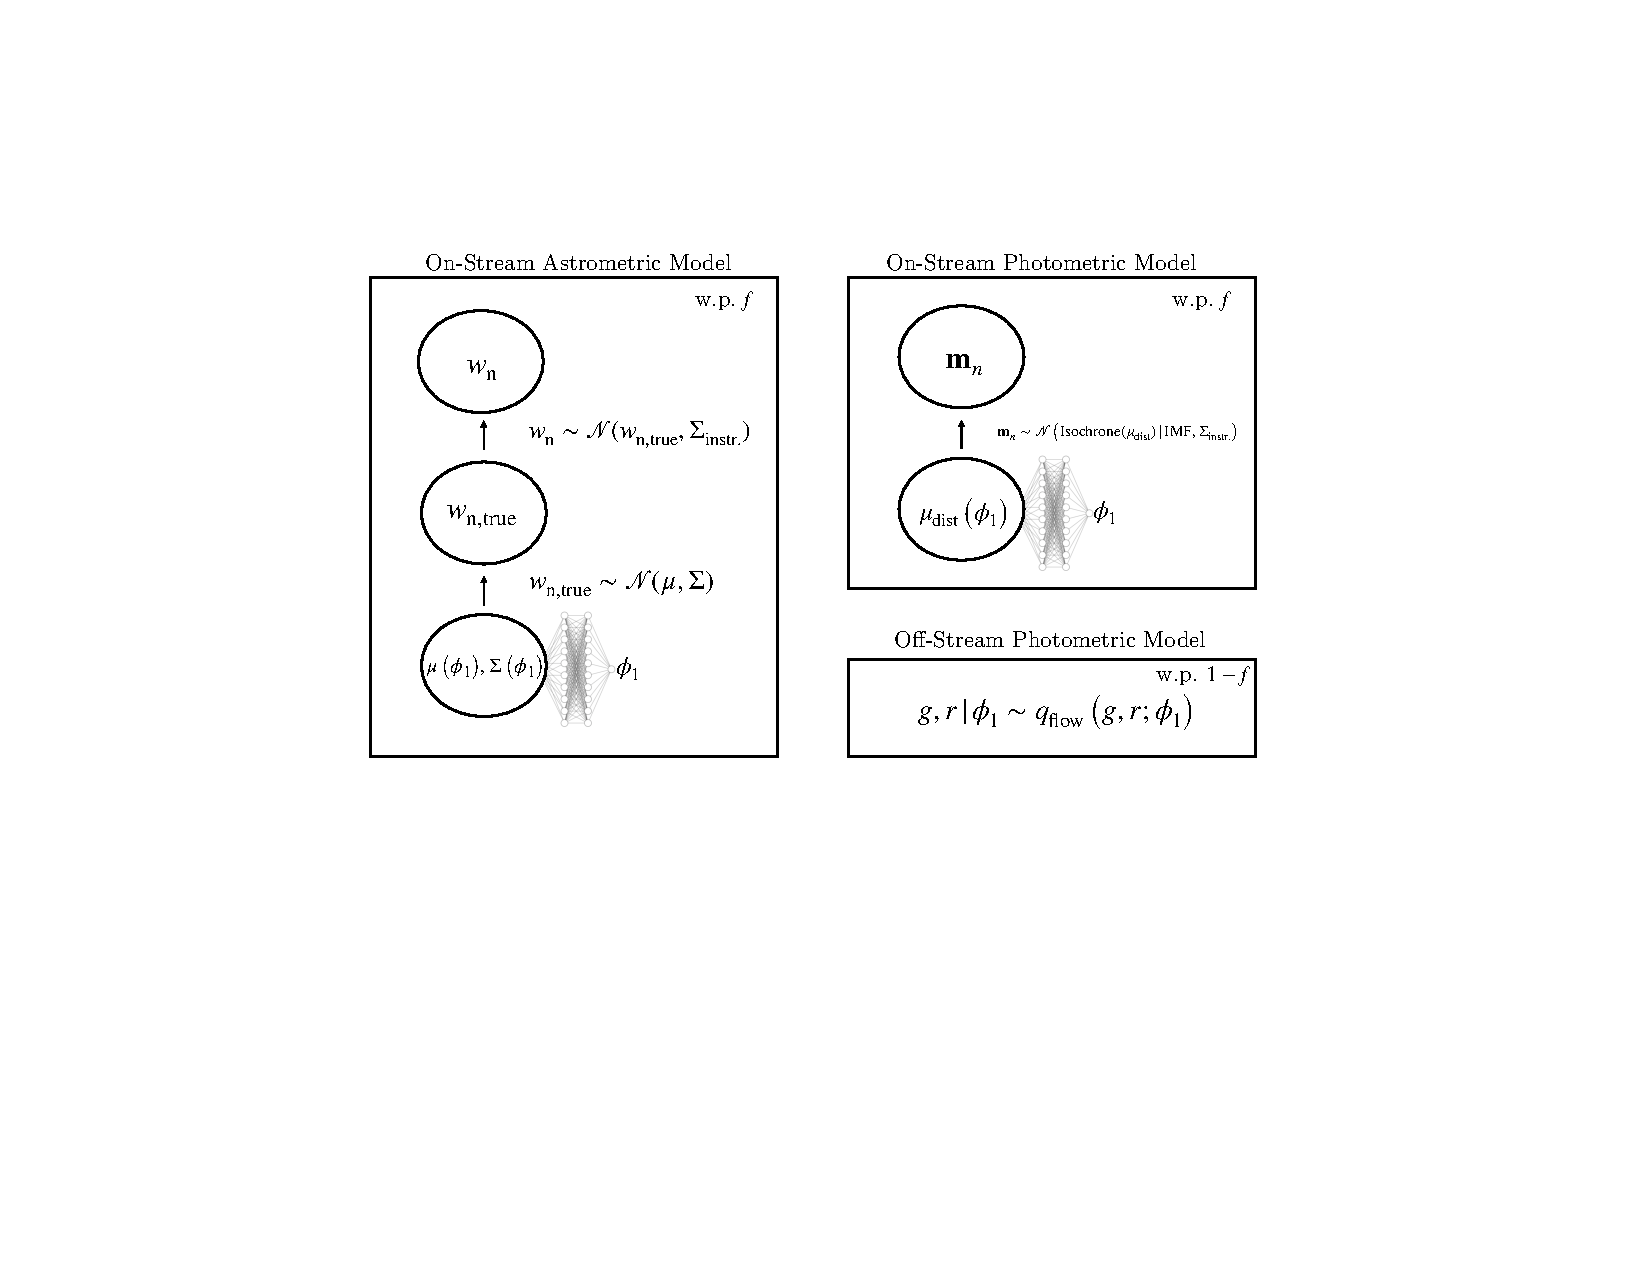
\includegraphics[scale=0.5]{static/DAG_StreamDensity.pdf}
            \caption{Fill in.}
            \label{fig: DAG}
        \end{figure}

        We model the likelihood for a single star as
        \begin{align} \label{eq:general_model}
            \pdf(\nth{\mbs{w}}, \nth{\mbs{m}} | \mbs{\theta})
                &= \sum_{q} \ f_q(w_{i, 0}) \pdf(\nth{\mbs{w}}|\mbs{\theta},q_i\!=\!q) \pdf(\nth{\mbs{m}}|\mbs{\theta},q_i\!=\!q)
        \end{align}
        where we have assumed that $\nth{\mbs{w}}$ and $\nth{\mbs{m}}$ are
        conditionally independent, and that the mixture weights $f$ are
        normalized s.t. $\sum_q f(w_{i,0}) = 1$.  We discuss the mixture weights
        further in \autoref{sub:mixture_weight}.

        Assuming the measurement of each star is independent, the total
        log-likelihood is a sum over all stars:
        \begin{equation}
            \ln\mcal{L}\left(\{(\nth{\mbs{w}},\nth{\mbs{m}})\} | \mbs{\theta}\right) = \sum_i  \ln \pdf(\nth{\mbs{w}}, \nth{\mbs{m}} | \mbs{\theta}).
        \end{equation}

        It will prove convenient to distinguish the models for $q=0,1$ as the
        \textit{background} and \textit{stream} models, respectively. In this
        notation:

        \begin{align}
            \pdf(\nth{\mbs{w}}, \nth{\mbs{m}} | \mbs{\theta})
            =& \phantom{+} \qquad f \phantom{+} P^{(S)}(\nth{\mbs{w}}|\mbs{\theta}) P^{(S)}(\nth{\mbs{m}}|\mbs{\theta}) \\
            & + (1-f) P^{(B)}(\nth{\mbs{w}}|\mbs{\theta}) P^{(B)}(\nth{\mbs{m}}|\mbs{\theta}), \nonumber
        \end{align}

        The probablity of a being a stream member is then simply
        \begin{equation}\label{eq:membership_prob}
            \pdf\left(S | \mbs{w}_n, \mbs{m}_n, \mbs{\theta} \right) = \frac{f P^{(S)}(\nth{\mbs{w}}|\mbs{\theta}) P^{(S)}(\nth{\mbs{m}}|\mbs{\theta}) }{ \pdf(\nth{\mbs{w}}, \nth{\mbs{m}} | \mbs{\theta})}.
        \end{equation}

        Hereafter, when we refer to ``membership probability,"
        \autoref{eq:membership_prob} provides the formal definition.


        \paragraph{missing phase-space observations}

            Streams have a diversity of measurement coverage: several have full 6-D astrometrics as well as photometrics and chemical abundances available \citep[e.g.,][]{Koposov2019, 2020A&A...635L...3A, 2022ApJ...928...30L}, while most have partial coverage, lacking feature dimensions.
            % TODO: terminology ND-phase-space vs feature columns
            Most streams in \dataarchive{Gaia} {\color{red} [cite]}, for instance, have proper motions but not radial velocities nor reliable parallax measurements. Followup surveys, like \dataarchive{S5} {\color{red} [cite]}, add many feature dimensions, however only for a select set of streams. Given the diversity of coverage it is important that the likelihood model can deal with missing data.

            The method of treatment of missing data depends on the cause for that data to be missing.
            Broadly, there are two categories of causes: randomness and systematics.
            Consider a dataset with all features measured but with a random subset of features masked.
            One possible approach is to attempt to impute the missing features, then feed the full-featured data to the likelihood model. Alternatively, the likelihood model might use only the present features, ignoring those missing. If however, features are missing for systematic reasons, then this approach can introduce systematic bias. Consider a star too far away to measure it's parallax distance or radial velocity. This is a systematic reason and this information should be incorporated into any model as a prior. Not doing so, the data imputation approach might predict too-close distances. Likewise, using only present features in the likelihood model misses that the star is likely very distant.

            {\color{red} Sentence explaining why we ignore features regardless.}
            We include a quality flag on our calculations, indicating the number of missing features.
            % TODO! in the table

            The per-star likelihood is modelled with a distribution with the same dimensionality as the data vector.
            For example, a star with a 6D astrometric measurement will be modelled with a full 6D distribution, while a star missing its radial velocity measurement, will be modelled with a 5D dimensionally-reduced form of the 6D distribution. Using dimensionally reduced distributions ensure that missing phase-space dimensions do not amplify nor suppress the likelihood.


    % subsection likelihood_setup (end)

    \subsection{Determination of the Mixture Weight} \label{sub:mixture_weight}
        The mixture weight $f_q(\phi_1)$ as used in \autoref{eq:general_model} is characterized as the fraction of stars belonging to the mixture component $q$ over an increment $[\phi_1, \phi_1 + \dif{\phi_1}]$. Thus, the mixture weight encodes information about the linear density of the stream, which has been shown to depend on substructure in the galaxy (CITE-x). The dependence of the mixture weight on the linear density is captured by the expression
        \begin{equation}\label{eq:fraction_param}
            f_q\left(w_{i,0}\right) = \frac{N_q\left(\phi_1\right)}{N_{\rm tot}\left(\phi_1\right)},
        \end{equation}
        where $N_q\left(\phi_1\right)$ is the number of stars in component $q$ within an interval $[\phi_1, \phi_1 + \dif{\phi_1}]$, and 
        $N_{\rm tot}$ is the total number of stars in the same band (including those in component $q$). The linear  density for component $q$ is then entirely specified by the function $N_q(\phi_1)$.

        The mixture model specified in \S-X only models the weight parameter $f_q$, and not the components of the ratio in \autoref{eq:fraction_param}. However, the linear density $N_q(\phi_1)$ can be readily obtained from $f_q$, provided that $N_{\rm tot}\left(\phi_1\right)$ can be calculated. Importantly, this function does not depend on the parameters of the on-stream or off-stream model. Instead, $N_{\rm tot}(\phi_1)$ is simply the number of stars in a small $\phi_1$ increment. We therefore model $N_{\rm tot}\left(\phi_1\right)$ as a post-processing step using a single normalzing flow in $\phi_1$. 

        In particular, for a given field the distribution of $\phi_1$ coordinates is specified by the set $\{\nth{\phi_{1}}\}_f$. A normalizng flow is trained to this dataset, and will satisfy $\int d\phi_1 P_{\phi_f}(\phi_1) = 1$ by construction. In order to re-weight the normalizing flow to obtain $N_{\rm tot}(\phi_1)$, we simply rescale $P_{\phi}(\phi_1)$ by $N_{\rm tot,0}$, which is the total number of stars in the field considered. We can then obtain the linear stream density with
        \begin{equation}
            N_q\left(\phi_1\right) = f_q N_{\rm tot} \left(\phi_1\right)  = f_q \left[N_{\rm tot,0} P_{\phi_1}\left(\phi_1\right) \right] .
        \end{equation}

    
        
    \subsection{Astrometric Model} \label{sub:astrometric_model}

        \subsubsection{On-Stream} \label{ssub:astrometric_model_on_stream}
    
            The astrometric track is modeled with a neural network, encompassing each phase space dimension, parameterized as a function of $\phi_1$. The neural network output for a single stream component is the mean location of the stream track in each dimension, $\astroM{\mbs{\mu}}(\phi_1)$, and its associated covariance matrix $\astroM{\mbs{\Sigma}}(\phi_1)$. The probability for the data is then
            \begin{equation}
                \pdf^{(S)}(\nth{\mbs{w}} | \astroM{\mbs{\theta}}(\nth{\phi_{1}})) = \mcal{N}_F \big(\nth{\mbs{w}} | \astroM{\mbs{\mu}} \left(\nth{\phi_{1}} \right), \astroM{\mbs{\Sigma}} \left(\nth{\phi_{1}}\right) \big),
            \end{equation}
            where $\mbs{\theta}$ is the set of neural network parameters that define $\astroM{\mbs{\mu}}$ and $\astroM{\mbs{\Sigma}}$.
            In the simplest case, we take $\astroM{\mbs{\Sigma}}$ to be diagonal, consisting of both intrinsic dispersion for each dimension of $\mbs{w}$ and the data uncertainties added in quadrature. 

            In practice, we work with truncated Gaussians, where the truncation is set by the size of the field in each astrometric dimension. Details of the truncated Gaussian are included in \autoref{app:sub:normal_distribution}. Truncating to the field ensures that the probability density is zero wherever there is no data. This has an added benefit of correctly normalizing the Gaussian distribution, which is not compact (has non-zero probability over all space) and would otherwise not integrate to one within the field.

            As a MDN, we implement the Gaussian distribution parameters with a multi-layered feed-forward neural network. The number of layers required depends on the maximum dimensionality of the Gaussian, and whether the neural network employs regularization techniques like dropout. We use alternating layers of linear and tanh units. Details of the network architecture are discussed in \autoref{sub:model_implementation}.

            In the presence of missing phase-space coordinate $f_k$ we reduce the dimensionality of the Gaussian to that of the data-vector. Namely, for $\mbs{I}_{\tilde{F}} = \mbs{I}_{F} \backslash f_k$
            \begin{align}
                \nth{\tilde{\mbf{w}}} &\mapsto \nth{\tilde{\mbf{w}}} = \{ w_{n,f}\}_{f\in \mbs{I}_{\tilde{F}}}, \nonumber\\
                \astroM{\mbs{\mu}} &\mapsto \astroM{\tilde{\mbs{\mu}}} = \{ \mu_{f}\}_{f\in\mbs{I}_{\tilde{F}}}, \nonumber\\
                \astroM{\mbs{\Sigma}} &\mapsto \astroM{\tilde{\mbs{\Sigma}}} = \{ \Sigma_{i,j}\}_{i,j \in \mbs{I}_{\tilde{F}}}, & \nonumber
                \intertext{such that,}
                \pdf^{(S)}(\nth{\mbs{w}} & | \astroM{\mbs{\theta}}(\nth{\phi_{1}}))
                    \mapsto \pdf^{(S)}(\nth{\tilde{\mbs{w}}} | \astroM{\tilde{\mbs{\theta}}} (\nth{\phi_{1}})).
            \end{align}

        \subsubsection{Off-stream} \label{ssub:astrometric_model_off_stream}
    
            We now outline the off-stream astrometric model. We take a similar approach to the on-stream astrometric model discussed in \autoref{ssub:astrometric_model_on_stream}, though we typically do not characterize the backgrounds with a Gaussian distribution. Instead, we utilize a range of distributions (i.e., exponential, skew-normal) discussed in \autoref{app:distributions}. The parameters of the user-specified background distributions are themselves neural network outputs, such that any $\phi_1$ ``slice" of the background should be characterized by some analytic density, but the evolution of the backgrounds with $\phi_1$ can be complex. Details of the network architecture are discussed in \autoref{sub:model_implementation}.
    
            Let $\fth{\cmp{B}{\mbs{\theta}}}(\phi_1)$ represent the neural network which outputs a vector of parameters characterizing the background distribution at a given $\phi_1$ for astrometric dimension $f$. The number of outputs for the background model is equal to $\mathrm{dim}\left(\fth{\cmp{B}{\mbs{\theta}}}\right)$ (where $f=0$ corresponds to $\phi_1$, which we do not model). At a given $\phi_1$, the probability density for the astrometric dimension $f>0$ is $\fth{\pdf^{(B)}}\left(\mbs{w}_{n,f} | \fth{\cmp{B}{\mbs{\theta}}}(\phi_1) \right)$. We treat each background component as independent, allowing us to write the likelihood as a product over the astrometric dimensions:
            \begin{equation} \label{eq:astrometric_model_off_stream_probability}
                \pdf^{(B)}\left(\nth{\mbs{w}} | \mbs{\theta}(\phi_1) \right) = \prod_{f\in \mbs{I}_{\tilde{F}}} \pdf_f^{(B)}\left(\mbs{w}_{n,f} | \fth{\cmp{B}{\mbs{\theta}}}(\phi_1) \right).
            \end{equation}
            Where $\mbs{I}_{\tilde{F}}$ is the set of indices of the features, omitting missing phase space dimensions.
        
    %\newpage

    \subsection{Photometric Model} \label{sub:photometric_model}

        \subsubsection{On-Stream} \label{sub:photometric_model_on_stream}
            In photometric coordinates we model the stream as a single-population isochrone with the possibility of a non-zero distance gradient. We accomplish this by modeling the distance of the isochrone as a neural network output, parametrized as a function of $\phi_1$. The result is a distance track along the stream, estimated from the variation in its isochrone with $\phi_1$. 
            
            At any given $\phi_1$, the isochrone is modeled in absolute magnitudes
            and parameterized by the unit-normalized stellar mass, labeled $\gamma$. For example, increasing $\gamma$ corresponds to movement up the main sequence towards the red giant branch. We denote the isochrone as $\mcal{I(\gamma)}$. The intrinsic dipsersion around the isochrone is $\Sigma_\mcal{I}(\gamma)$. Since the isochrone is in absolute magnitudes, but the data are in apparent magnitudes,
            it is necessary to shift the isochrone by a distance modulus to the predicted distance of the stream, labeled  $\mu(\nth{\phi_1})$.
            
            For the $n$-th star, the photometric model is:
    
            \begin{multline}
                P^{(S)}(\mbs{m_i}, \gamma; \mbs{\theta}(\nth{\phi_1}), \nth{\phi_1}) 
                \\ \sim \mcal{N}(\nth{\mbs{m}}; \{\mcal{I(\gamma)} + \mu(\nth{\phi_1}), \sqrt{\Sigma_{\mcal{I}}^2(\gamma) + \Sigma_\mu^2(\nth{\phi_1}) + \Sigma_i^2} \}) \\ \times\pdf(\gamma, \nth{\phi_1}),
            \end{multline}
    
            where $\pdf(\gamma)$ encodes both the present-day mass function of the stream, as well as the observational constraints (e.g. $g < 22$ mag).
    
            We are interested in the total probability (at some $\phi_1$) and so integrate over $\gamma$ to find:
            \begin{small}
            \begin{multline}
                P^{(S)}(\nth{\mbs{m}}; \mbs{\theta}(\nth{\phi_1}), \nth{\phi_1}) = \\\int\limits_{\gamma=0}^{1} \mcal{N}(\mbs{m}; \{\mcal{I(\gamma)} + \mu(\nth{\phi_1}), \sqrt{\Sigma_{\mcal{I}}^2(\gamma) + \Sigma_\mu^2(\nth{\phi_1}) + \Sigma_i^2} \}) \pdf(\gamma) \rm{d}\gamma.
            \end{multline}\end{small}
            Then, for a given $\phi_1$ we can obtain a distribution over the distance modulus using 
            \begin{equation}
                \mu_{\rm sample}\left(\phi_1\right) \sim \mathcal{N}\left(\mu(\phi_1), \Sigma^2_\mu(\phi_1) \right) \quad\unit{mag}.
            \end{equation}
            For each sample, we can convert the distance-modulus distribution to the distance track using 
            \begin{equation}
                \rm{dist}\left(\phi_1\right) = 10^{\frac{1}{5}\mu_{\rm sample}(\phi_1)+1} \quad\unit{pc}.
            \end{equation}

            

            \todo[inline]{TODO:}
            \begin{enumerate}
                \item Not including isochrone parameters, e.g. age and metallicity
                \item integrating over $\gamma$ the model assumes a PDMF, e.g. Kroupa
                \item generic details of neural network, e.g Table 1
                \item introducing parallax
                \item how we reduce dimensionality.
            \end{enumerate}

    
        \subsubsection{Off-stream} \label{sub:photometric_model_off_stream}
            In this section we introduce our model for the distribution of backgrounds in photometric coordinates. 

            In general, the distribution of stars in color (i.e., $g-r$) and magnitude (i.e., $g$) is a complicated function of location in the galaxy. Even within a field centered on the stream of interest, the color-magnitude diagram (CMD) is a combination of stellar populations distributed over a range in distances. Because of this, we do not expect an analytic density to provide a realistic description of the data. In this work we take a data-driven approach, and represent the CMD using a normalizing flow model.

            Normalizing flows provide a flexible description of a probability density, by transforming samples generated from a simple base distribution (i.e., a Gaussian) to the more complicated target distribution. The transformations are typically non-linear outputs of a neural neural network, whose parameters are optimized until the target density accurately characterizes the data. The neural network transformation is differentiable, so that jacobian factors can be combined to ensure that the the target distribution remains a valid probability density (i.e., integrates to one).  

            Our implementation is as follows. For a given stream, we restrict the data to some field characterized by a polygon drawn around the stream. Because our density modeling is aimed at stream characterization rather than discovery, we assume that the stream is sufficiently well known so that it can be masked out as a simple cut in (e.g.) $\phi1-\phi_2$ coordinates. With the stream masked out, we then fit a normalizing flow to the photometric data. Because the background CMD can evolve with $\phi_1$, we fit a \emph{conditional} normalizing flow, $q_{\rm flow}(\mathbf{m}|\phi_1)$, so that the color-magnitude diagram is conditionally dependent on position along the stream. In practice, we model magntiudes and not colors (i.e., $\mathbf{m} = (g,r)$ rather than $g \ \mathrm{and} \ g-r$. Otherwise, the two arguments will always be covariate). Our central assumption with this model is that the distribution of colors and magnitudes for background stars in the masked region are quantitatively similar to those in the unmasked region. For a sufficiently narrow mask we expect this to be the case, and find that this assumption does not introduce bias for the streams considered in this work.
                
            Once the normalizing flow, $q_{\rm flow}\left(\mathbf{m} | \phi_1\right)$, is fit to the data, its parameters are fixed while the other components of the model begin training. Therefore, the normalizing flow can be rapidly trained and computed as a pre-processing step. 

            The specific architecture of the photometric normalizing flow are discussed in \S-X.

            \todo[inline]{TODO:}
            \begin{enumerate}
                \item Overview of the architecture
                \item How one would reduce the dimensionalty.
            \end{enumerate}

            
    % subsection likelihood_setup (end)

    % \vspace{10pt}

    % \subsection[Astrometric Background]{Astrometric Background: pieces of $P^{(B)}(\mbs{w})$} \label{sub:background_astrometric}

    %     When looking for a stellar stream, the highly complex Galaxy is the background. There are numerous approaches to modeling a complex structure, from a mix of very simple models to a single highly flexible model, like a basis function expansion or ML network.
    %     We aim towards the mix of simple models, but use more flexible models as needed. In this section we describe the various models used when modeling the background, in different coordinates of the phase space.

        % \subsubsection{Flat Background} \label{ssub:flat_background}

        %     The simplest possible background is the flat background.
        %     Perhaps surprisingly, the Galaxy around GD-1 is well modeled by a flat distribution in the $\phi_2(\phi_1)$ phase space.
        %     For a domain $x \in [a, b]$ the normalized PDF is given by
        %     \begin{align}
        %         \pdf(x|a,b) &= \frac{1}{b-a} & \text{and} \\
        %         \ln \pdf(x | a, b) &= -\ln\left({b-a}\right)
        %     \end{align}
        %     where $a,b$ are the $\phi_2$ bounds of the data selection box.
    
        % % subsubsection flat_background (end)

        % \subsubsection{Exponential-like Background} \label{ssub:exponential_background}

        %     In many coordinate axes, the distribution of the background data is better described by an exponential distribution.
        %     The unit-normalized exponential distribution in the domain $[a, b]$ ($a \neq b$) is given by:
        %     \begin{equation}\label{eq:exp_distr}
        %         f(x) = \frac{m \Exp{-m (x - a))}}{1 - \Exp{-m(b - a)}}.
        %     \end{equation}
        %     However for $m \rightarrow 0$, which describes the flat distribution (\autoref{ssub:flat_background}), this functional form can be numerically unstable, particularly with lower bit precision numerics like \texttt{float32} data-types. In the context of ML, the numerical instability is problematic when employing parameter drop-out for $m$. While for parameter dropout this might be avoided by re-parameterizing to $m+\epsilon$, the numerical instability remains and may be encountered later, creating a difficult-to-diagnose \texttt{NaN}. 
        %     For both compatibility with the flat distribution and for practical reasons we modify the above distribution and approximate the exponential distribution with a 3rd order expansion around $m=0$ when $|m| < \epsilon$, for some small $\epsilon$.

        % % subsubsection exponential_background (end)

        %% PLOT HERE OF ALL THE BACKGROUNDS?? **

    % subsection astrometric background (end)

        

        % Let $\Omega$ be the independent variable in $\mbf{w}$.

        % $\pdf(m_i | ) \rm{KDE(\mbf{m}_i|\omega_{i} )}$

    % subsection photmetric background (end)

        \begin{figure}
            \script{mock/plot/photometric_background_selection.py}
            \centering
            \includegraphics[width=1\linewidth]{figures/mock/photometric_background_selection.pdf}
            \caption{Caption: TO-DO need to show this with a ground truth (e.g. show true weight in top panel).}
            \label{fig:mock_data_photometric_background_selection}
        \end{figure}

        \begin{figure*}
            \script{mock/plot/results.py}
            \centering
            \includegraphics[width=1\linewidth]{figures/mock/results.pdf}
            \caption{Caption: .}
            TODO:
            \begin{enumerate}
                \item Get rid of the dropout in the plot
                \item the linear density in the stream-fraction plot
            \end{enumerate}
            \label{fig:mock_data_result}
        \end{figure*}

    \subsection{Priors} \label{sub:priors}

        \subsubsection{Bounding Boxes}


        \subsubsection{Region Prior} \label{sub:track_region_prior}

            Region priors encourage the model to pass through a user-defined control region, while also remaining compatible with the data.

            The overall track of the stream is known, so it makes sense to give this information to the system. However, we don't want the prior to dominate the results on small scales. A good balance between these two goals is to have a prior that only influences the track on large scales.
            We introduce the ``split" Gaussian prior, which is a Gaussian split at the peak and pieced back together with a flat region connecting the halves. 
            It is smooth up to the first derivative, so works well in an auto-grad setting.
            The unnormalized PDF is described by:
            \begin{small}
            \begin{equation}
                \pdf(x,\mu,\sigma,w) \propto  \frac{1}{\sigma \sqrt{2 \pi}} \begin{cases} 
                   \Exp{-\frac{1}{2}\left(\frac{x-(\mu-w)}{\sigma}\right)^2} & \phantom{\mu - w <}\ x < \mu - w \\
                    1 & \mu - w \leq x < \mu + w \\
                    \Exp{-\frac{1}{2}\left(\frac{x-(\mu+w)}{\sigma}\right)^2} & \mu + w < x
                \end{cases}.
            \end{equation}\end{small}
    
            Since this prior is equi-probable in the region $\mu - w < x < \mu + w$, the  impact is to encourage the stream to fall anywhere within this region. 
            It is convenient to reparametrize, with $\tau = \frac{1}{\sigma}$.
            \begin{small}
            \begin{equation}
                \ln \pdf(x,\mu,w) \propto \tau \begin{cases} 
                    -\left(x-(\mu-w)\right)^2 & \phantom{\mu - w <}\ x < \mu - w \\
                    0 & \mu - w \leq x < \mu + w \\
                    -\left(x-(\mu+w)\right)^2 & \mu + w \leq x
                \end{cases},
            \end{equation}\end{small}
            where the additive normalization is 
            $-\ln\left(\sqrt{\frac{\pi}{\tau}} \left(\frac{1}{2}\text{erf}\left(2 \sqrt{\tau } w\right)+1\right)\right)$


    \subsection{Linking Coordinates: Combining the Distance Modulus with the Parallax Track}

        \todo[inline]{TODO:}
        \begin{enumerate}
            \item Discuss how to connect the distance modulus to the parallax.
            \item First-order error propagation to set width DM to width parallax.
        \end{enumerate}


    \subsection{Model Implementation, aka the code} \label{sub:model_implementation}

        \todo[inline]{TODO:}

        \begin{enumerate}
            \item A network per model component, e.g. one for the weights, one for the stream track and width, one for the background distribution.
            \item MLP for the components - lin / tanh + dropout
            \item Normalizing flow - specific pieces
            \item Architecture in the Appendix
        \end{enumerate}


        \begin{table}
            \centering
            \caption{MLP structure}
            \begin{tabular}{@{}rrcl@{}}
            \toprule
            & Layer & Shape & Param \# \\
            \midrule
            & Linear & (None, 1, F) & 1  \\
            & Tanh & (None, 1, F) & 1  \\
            & Dropout & (None, 1, F) & 0  \\
            & Linear & (None, 1, F) & 1  \\
            \bottomrule
            \end{tabular}
        \end{table}


        Dropout layers were used to prevent network co-adaptation and over-fitting. Droput works by randomly zeroing out nodes in the network, decreasing the importance of single nodes versus emergent patterns across the  network.

        
% section method (end)

%\newpage
\section{Results} \label{sec:results}

    In this section we present an application of our model to a synthetic stream with known ground truths, and demonstrate the model's ability to characterize stream density variations and membership probabilities in an unsupervised manner. We then apply the method to real stellar streams in \autoref{sub:gd1} and \autoref{sub:pal5}.

    \subsection{Test on a Synthetic Stream} \label{sub:mock_data}
    
        In this section we apply our model to a synethic stream in order to demonstrate an accurate recovery of stream members and density variations.
    
        We generate synthetic observations by sampling points from a third degree polynomial \JN{check this} with a constant scatter. Density variations are then simulated by evaluating the stream density with two Gaussian distributions centered at different values of $\phi_1$ with random amplitudes (which sum to $1$) and widths. Stream stars are then removed using random sampling, weighted by their likelihood of belonging to the density. The background astrometric  points in are generated from exponential distributions at each $\phi_1$. The number of stream stars is \JN{X}, while the number of background stars is \JN{Y}.
    
        The synthetic stream is also simulated in magnitudes using a 12~Gyr isochrone with [Fe/H] = -1.35~dex. The isochrone truncates just short of the giant branch, and sampled from uniformly (i.e., the initial mass function, $P(\gamma)$, is uniform). The background photometric coordinates are generated as a 2-dimensional Gaussian with non-zero covariance. The distance modulus is derived from a polynomial parallax track with uniform thickness. Thus, the synthetic data scenario described here generates a mock stream in astrometric coordinates and photometric coordinates, with density variations, a distance gradient which is consistent in parallax and distance modulus (i.e., magnitudes), all superimposed over a noisy field of background points in each astrometric and photometric dimension.
    
        The result of applying our density model to the synthetic data is illustrated in \autoref{fig:mock_data_result}. The top panel shows the weight parameter that controls membership probability as a function of $\phi_1$. The dashed curve represents the output of our data-driven model, while the solid curve is the ground truth. \JN{todo: maybe the kde should be a histogram}, the second panel shows the stream and background in the $(\phi_1,\phi_2)$ plane, and the third panel shows the stream and background in the $(\phi_1,\varpi)$ plane. Points are color-coded according to their membership probability (Eq.~X) \JN{would be good to remove the $\sigma$ bands in this plot.} The weight parameter clearly shows that the model has captured the two prominent density variations along the stream. The are additional variations  mostly around the edges of the stream, though re-sampling the neural network weights with dropout reveals that these variations represent regions of higher model uncertainty. 
        
        We find that the stream is successfully recovered in both astrometric and photometric coordinates, with $x\%$ stream stars being recovered with membership probability greater than $y$. The false positive rate (i.e., stars misidentified as stream members) for this test is found to be $z\%$ when cutting on this threshold. 
    
        In the bottom two rows of \autoref{fig:mock_data_result} we illustrate the synthetic data color-coded by stream membership probability (top) and background membership probability (background) for different $\phi_1$ slices. Importantly, the photometric portion of the mixture model successfully identifies the stream in magnitude space, showing a high stream membership probability where the stream is present, and a low probability ($\sim 0$) where the stream is absent.  
    
    % subsection test_on_a_synthetic_stream (end)
    
    \subsection{Results on GD-1} \label{sub:gd1}

        We now apply our density modeling approach to the stellar stream GD-1. We discuss the data selection in \autoref{ssub:gd1_data} and results in \autoref{ssub:trained_gd1}.
        
        \subsubsection{Data Selection} \label{ssub:gd1_data}
            We utilize data from {\it Gaia} DR3 for the astrometric coordinates of each star, and Pan-STARRS1 to obtain more accurate color information. We adopt broad cuts on the cross-matched data to limit the field to a region known to contain GD-1. We perform these rough cuts by requiring \JN{fill in what the cuts are and reference proper motion figure and CMD figure.} 

            The result is a field populated by \JN{x} stars, from which we would like to identify stream members.

        \subsubsection{Model Specification}\label{sec:GD_1_ModelSpecification}
    
            We model GD-1 as a three-component mixture consisting of a main stream component, a spur, and background. In order to guide our model towards GD-1, we set down 4 ``control points" along GD-1's main track, and 3 control points along the spur (illustrated in \JN{x}). These control points act as gaussian priors on the model. We set the Gaussian error on these control points to large values, so that their influence on the model is not dominant. Indeed, we find that the value of the control points is to help reduce training time, since otherwise it will take the flexible density model longer time to converge to the actual stream.
    
            The weight parameter is also set to truncate to $0$ at $\phi_1 < X$ and $\phi_1 > Y$. This ensures that we do not model stream stars that fall 
        
        
        \subsubsection{Trained Density Model}\label{ssub:trained_gd1}
    
            In this section we present results from our model applied to real {\it Gaia} and Pan-STARRS data of GD-1. 

            We visualize the performance of our model in identifying stream stars and characterizing the astrometric background with \autoref{fig:gd1-results-full} and \autoref{fig:gd1-results-panels}. In \autoref{fig:gd1-results-full} The top panel shows the stream in $\phi_1$, $\phi_2$ coordinates, color-coded by membership probability (derived from \autoref{eq:membership_prob}). The following three rows represent background distributions in $\phi_2, \mu_{\phi_1}, \rm{\ and} \ \mu_{\rm phi_2}$, respectively taken at different $\phi_1$ increments centered on the red lines. The $\phi_1$ increments are roughly $\sim X$ in size. 

            The blue lines over-plotted represent the best fit model at the given $\phi_1$ slice. We find that the backgrounds are typically well characterized by the distributions adopted (described in \S-x). We can also see from \autoref{fig:gd1-results-panels}
            that the stream and spur components appear to be well characterized. 
            
            Our ability to recover the stream is demonstrated further in \autoref{fig:gd1-results-full}. In this figure, we only plot stars if their membership probability is greater than \JN{X}. The result is a ``gold" catalog of probable stream and spur members, extending over $X$-degrees in $\phi_1$. We find the expected gap around $\phi_1 \sim -20~\rm{deg}$, which has been proposed to be the location of the dissolved progenitor (CITE).

            Our model also fits the distribution of stream stars in the CMD. These fits are illustrated in \autoref{fig:gd1-results-panels}, where the CMD for the population in a given $\phi_1$ band is plotted, color-coded by stream membership probability. For the on-stream regions, the isochrone appears to provide a decent description of the stream, though there is room for further improvements (discussed in \S-x). However, we note that the stream's presence and absence in the isochrone is well captured by the mixture weight, which is a neural network output. 
            
            Additionally, the distance modulus is also a neural network output, conditioned on $\phi_1$. This allows us to obtain a distance modulus at each $\phi_1$ along the stream. The distance modulus track and (converted) distance track are illustrated in \autoref{fig:gd1-results-full}. The left panel shows the distance modulus (in magnitudes), while the right shows the corresponding distance track. Importantly, the prior on the distance track is that the stream must fall between $[4,40]~\rm{kpc}$. Thus, our ability to recover the distance to GD-1 without substantial bias provides a useful indicator that our color-magnitude model combined with the astrometric model provide an adequate description of the data. \JN{more on this...}

            \begin{figure*}[h]
                \script{gd1/plot/data_selection.py}
                \centering
                \includegraphics[width=1\linewidth]{figures/gd1/data_selection.pdf}
                \caption{Caption}
                \label{fig:gd1-data_selection}
            \end{figure*}

            \begin{figure}
                \script{gd1/plot/photometric_background_selection.py}
                \centering
                \includegraphics[width=1\linewidth]{figures/gd1/photometric_background_selection.pdf}
                \caption{Caption}
                \label{fig:gd1-photometric_background_selection}
            \end{figure}

            \begin{figure*}[h]
                \script{gd1/plot/results_full.py}
                \centering
                \includegraphics[width=1\linewidth]{figures/gd1/results_full.pdf}
                \caption{CAPTION}
                TODO:
                \begin{itemize}
                    \item Add plot of the stream linear density
                    \item Color palette for the spur
                    \item more subtle stream MLE path
                    \item rerun model with larger pmphi2 sigma
                    \item add the isochrones to the cmd plots
                \end{itemize}
                \label{fig:gd1-results-full}
            \end{figure*}

            \begin{figure*}[h]
                \script{gd1/plot/results_panels.py}
                \centering
                \includegraphics[width=1\linewidth]{figures/gd1/results_panels.pdf}
                \caption{CAPTION}
                TODO:
                \begin{itemize}
                    \item Add plot of the stream linear density
                    \item Color palette for the spur
                    \item add the isochrones to the cmd plots
                \end{itemize}
                \label{fig:gd1-results-panels}
            \end{figure*}
    
            \begin{figure*}
                \script{gd1/plot/smooth_likelihood.py}
                \centering
                \includegraphics[scale=0.8]{figures/gd1/smooth_likelihood.pdf}
                \caption{Caption}
                \label{fig:gd1-heatmap}
            \end{figure*}

            \variable{output/gd1_select_members.tex}


    % subsection gd1 (end)

    \subsection{Palomar 5} \label{sub:pal5}

        Content

    % subsection pal5 (end)

% section results (end)


\section{Comparison to Other Methods} \label{sec:comparison}

    \subsection[STREAMFINDER]{\cite{2018MNRAS.477.4063M}}

        

    % subsection streamfinder (end)

    \subsection{VIA MACHINAE}{\cite{2022MNRAS.509.5992S}}

    % subsection via_machinae (end)

    \subsection[Uniform Modeling of 13 Stellar Streams]{\cite{PatrickEtAl2022}}

    % subsection uniform_modeling_of_13_stellar_streams (end)


\section{Conclusions} \label{sec:conclusions}


% section comparison_to_other_methods (end)


\section{acknowledgements}

    We would like to thank the Academy.

    \todo[inline]{reword}
    "This study was carried out using the reproducibility software
    \href{https://github.com/showyourwork/showyourwork}{\showyourwork}
    \citep{Luger2021}, which leverages continuous integration to
    programmatically download the data from
    \href{https://zenodo.org/}{zenodo.org}, create the figures, and
    compile the manuscript. Each figure caption contains two links: one
    to the dataset stored on zenodo used in the corresponding figure,
    and the other to the script used to make the figure (at the commit
    corresponding to the current build of the manuscript). The git
    repository associated to this study is publicly available at
    \url{https://github.com/mathren/CE_accretors}, and the release
    v.2.1 allows anyone to re-build the entire manuscript. The datasets
    are stored at \url{https://doi.org/10.5281/zenodo.7343715}, including
    the template setup to recreate them using MESA (version 15140 and
    the software development kit \texttt{x86\_64-linux-20.12.1}) and
    the scripts used to produce the figures."

    \paragraph{Software (alphabetical)}

        \package{asdf} \citep{Greenfield2015},
        \package{astropy} \citep{Astropy2013, Astropy2018, Astropy2022},
        \package{astroquery} \citep{Astroquery2019},
        \package{Matplotlib} \citep{Hunter2007},
        \package{NumPy} \citep{Harris2020},
        \package{Pytorch} \citep{Pytorch2019},
        \package{SciPy} \citep{Scipy2020},


\section*{Data Availability} \label{sec:data_availability}

    This study was carried out using the reproducibility software
    \href{https://github.com/showyourwork/showyourwork}{\showyourwork}
    \citep{Luger2021}, which uses continuous integration to
    programmatically download the data, perform the analyses, create the
    figures, and compile the manuscript. Each figure caption contains two links:
    one to the dataset used in the corresponding figure, and the other to the
    script used to make the figure. The datasets are stored at
    \todo[inline]{zenodo url}. The git repository associated
    with this study is publicly available at \todo[inline]{GitHub url}.

% section data_availability (end)


\bibliography{bib}

\appendix

\section{Notation} \label{app:notation}

    In this work we use multiple data sets and a variety of mathematical tools to analyze the data, including machine learning algorithms and statistical models.
    For clarity and to connect related components of the models used in this work, a consistent mathematical notation is crucial. Here we establish the notation and symbols used throughout this work.
    \autoref{table:symbol_table} enumerates the symbols used for the statistical models and the different datasets, e.g. distinguishing astrometric from photometric data. 

    \begin{table}
    \centering
    \caption{Symbol Table}
    \label{table:symbol_table}
    \begin{tabular}{p{0.35\linewidth} p{0.6\linewidth}}
    Symbol                         & Explanation \\
    \toprule
    % -----------------------------------------------------------------------------
    \\
    \multicolumn{2}{l}{\textbf{Datasets}:} \\
    \midrule
    % -------------------------------------------------
    \multicolumn{2}{l}{\textbf{Full Data}:}  \vspace{5pt} \\
    $\mbf{X} \in \mbb{R}^{(N, F+1)}$ & Full dataset.  \\
    $N$ & The number of independent measurements (aka stars) in the dataset.  \\
    $F$ & The number of measured features, e.g. $(\alpha, \delta, \varpi, \mu_{\alpha^*}, \mu_\delta, v_r, g, r)$,  not including the the `independent' feature over which the others are conditioned. \\
    $\mrm{n} \in \mbs{I_N} \equiv \{1, ..., N\} \in \mbb{Z^+}$ & Index into the set of measurements $\mbf{X}$. \\
    $\mrm{f} \in \mbs{I_F}  \equiv \{1, ..., F\} \in \mbb{Z^+}$ & Index into the set of features of $\mbf{X}$. $ f=0$ is the `independent' feature.\\
    $x_{\mrm{n,f}}$ & $n$-th measurement of the $f$-th feature of $\mbf{X}$. \\
    $\nth{\mbs{x}}$ & $n$-th row-vector of all features. \\
    % -------------------------------------------------
    \\
    \multicolumn{2}{l}{\textbf{Astrometric Data}:}  \vspace{5pt} \\
    $\mbf{W} \in \mathbb{R}^{(N, F_w + 1)}$ & Full astrometric dataset. \\
    $\mrm{f_w} \in \mbs{I_{F_w}} \equiv \{1, ..., F_w\} \in \mathbb{Z^+}$ & Index into the set of astrometric features. $f_w = 0$ is the `independent' feature.\\
    $w_{\mrm{n,f_w}}$ & $n$-th measurement of the $f_w$-th feature of $\mbf{W}.$\\
    $\nth{\mbs{w}}$ & $n$-th row-vector of all astrometric features. \\
    $\phi_1 \equiv w_{\cdot,0}$ & The `independent' (index 0) feature column on which the models are conditioned.\\
    % -------------------------------------------------
    \\
    \multicolumn{2}{l}{\textbf{Photometric Data}:}  \vspace{5pt} \\
    $\mbf{M} \in \mathbb{R}^{(N, F_m)}$ & Full photometric dataset. \\
    $\mrm{f_m} \in \mbs{I_{F_m}} \equiv \{1, ..., F_m\} \in \mathbb{Z^+}$ & Index into the set of photometric features. \\
    $m_{\mrm{n,f_m}}$ & $n$-th measurement of the $f_m$-th feature of $\mbf{M}$. \\
    $\nth{\mbs{m}}$ & $n$-th row-vector of all features. \\
    % -----------------------------------------------------------------------------
    \\
    \multicolumn{2}{l}{\textbf{Statistics}:} \\
    \midrule
    $\pdf(...)$ & The PDF of the distribution. \\
    $\cdf(...)$ & The CDF corresponding to $\pdf(...)$. \\
    $\mbs{\theta} = \{\theta_f\}_f$ & The vector of a distribution's parameters. \\
    $\mcal{L}(\nth{\mbf{x}}, \mbs{\theta}(\phi_1))$ & The likelihood of the data given the parameters. \\
    $Q$ & The number of models in a mixture model. \\
    $\mrm{q} \in \mbs{I_Q} \equiv \{1, ..., Q \} \in \mbb{Z^+}$ & Index into the set of $Q$ models. \\
    % -------------------------------------------------
    \\
    \end{tabular}
    \end{table}

    We use $\tilde{F}$ to indicate that there a missing features, e.g. radial velocities.
    The index set $\mbs{I}_F \mapsto \mbs{I}_{\tilde{F}} = \{1, ..., k-1, k+1, ... \}$ where $k$ is the index of the missing feature.

% section notation (end)


\section{Theory of Mixture Density Networks (MDNs)} \label{app:theory_of_mixture_density_networks}

    Mixture models (MMs) are a statistical method to represent a population as a set of a sub-populations specified by probability distributions. These distributions are characterized by their parameters and mixture by a corresponding set of mixture weights. Mixture Density Networks (MDNs) 
    are a machine learning method to combine a MM with neural networks, increasing the flexibility of the model. An MDN replaces the scalar distribution parameters of the MM with neural networks, allowing the distribution parameters and mixture weights to vary as smooth functions \citep{Bishop1994}. Functional parameters allows the model to capture variation over those parameters that is not possible with scalar-valued models. Moreover, by using neural networks the inferred functional forms are ``model-free" and driven entirely by the data.

    % Quote from https://mikedusenberry.com/mixture-density-networks
    % A mixture density network (MDN) is an interesting model formalism built within the general framework of neural networks and probability theory for working on supervised learning problems in which the target variable cannot be easily approximated by a single standard probability distribution. Essentially an MDN allows one to model a conditional probability distribution as a mixture of distributions, in which the individual distributions and the corresponding mixture coefficients are parameterized by functions of the inputs 

    For the MDN we take $x_{\cdot, 0} \equiv x_{\cdot}$ (indexed from 0), which is the first feature column of $\mbf{X}$, as the `independent' coordinate over which the MDN parameters are conditioned. In the context of streams $x_{\cdot, 0} \equiv \phi_1$ is the longitude coordinate in a reference frame rotated such that the stream is aligned along $\phi_1$.

    The PDF of the MDN is

    \begin{equation} \label{eq:general_mixture_network}
        \pdf(\nth{\mbs{x}} | \mbs{\theta}(\phi_1))
        = \sum_{\mrm{q} \in \mbs{I_Q}} \ \qth{f}(\phi_1) \qth{P}(\nth{x}|\qth{\mbs{\theta}}(\phi_1),q\!=\!\mrm{q})
    \end{equation}
    The mixture coefficients $\qth{f}$ are normalized s.t.
    \begin{equation}
        \sum_{\mrm{q}} \qth{f}(\phi_1) = 1 \qquad \forall \phi_1
    \end{equation}
    In practice this is enforced by defining
    \begin{equation}
        f_{b}(\phi_1) = 1 - \sum_{\rm{q}\in \mbs{I_Q}\backslash b} \qth{f}(\phi_1)
    \end{equation}
    for some ``background" index $b \in \mbs{I_Q}$.

    Assuming the measurement of each datum is independent, the likelihood is a sum over all data:
    \begin{equation}
        \mcal{L}\left(\mbf{x}_n | \mbs{\theta}(\phi_1)\right) = \sum_{q\in\mbs{I_Q}} \qth{P}\left(\nth{\mbs{x}} | \qth{\mbs{\theta}}(\phi_1)\right).
    \end{equation}

    The full posterior distribution includes the priors.

    \begin{equation}
        \ln\posterior\left(\mbf{X} | \mbs{\theta}(\mbs{x})\right) = \ln\mcal{L}\left(\mbf{X} | \mbs{\theta}(\mbs{x})\right) +  \sum_{n \in \mbs{I_N}} \ln \left[ \sum_{q\in\mbs{I_Q}} \qth{\prior}\left(\qth{\mbs{\theta}}(\mbf{x}_n)\right) \right].
    \end{equation}


\section{Probability Distributions} \label{app:distributions}

    A variety of probability distributions are used when modeling the stream and Galactic background. This appendix presents relevant mathematical details of these distributions.
    In particular, observational errors are modeled as Gaussian distributions, which requires modifying each distribution to account for the Gaussian noise.

    \vspace{10pt}

    Let $x \sim X$ be distributed as some specified distribution
    and $\delta \sim \Delta \equiv \mcal{N}(0, \sigma_*)$ as an independent, centered Gaussian.
    An observation $Y$ is distributed as
    \begin{equation}
        Z = X + \Delta,
    \end{equation}
    Which is a convolution of the PDFs.
    \begin{align}  \label{eq:general_convolution}
        \pdf_Z(x; \mbs{\theta}, \sigma)
            & \equiv (\pdf_X(x; \mbs{\theta}) * \mcal{N}(x; 0, \sigma)) \\
            &= \int_{-\infty}^{\infty} \rm{d}\tau \, \pdf(x; \mbs{\theta})\mcal{N}(x-\tau; 0, \sigma)
    \end{align}

    In the following subsections we work through the distributions $\pdf(x,\mbs{\theta})$ and the convolutions with $\mcal{N}(x,0,\sigobs)$.

    \vspace{5pt}
    \subsection{Flat Distribution} \label{sub:flat_distribution}

        The simplest distribution is that of the univariate uniform distribution.
        For a domain $x \in [a, b]$ the PDF is given by
        \begin{equation}\label{eq:pdf_flat_univariate}
            P_{\mcal{U}}(x|a,b) = \begin{cases}
                (b-a)^{-1} & a < x \leq b \\
                0 & \text{else}
            \end{cases}
        \end{equation}
        where $a,b$ are the bounds.

        In practice, the bounds $a,b$ are the bounds of the observation window, creating a subset of a larger field.
        Suppose the larger field is uniformly distributed in a region larger than the bounds $a, b$, ie. $P_{\mcal{U}}(x|\alpha,\beta)$.
        Let each observed datum $x_n$ in the field have Gaussian error $\sigobs_n$,
        then the PDF of the uniform-Gaussian-convolved distribution is given by:

        \begin{equation}
            \pdf_{(\mcal{U}*\mcal{N})}(x; \alpha, \beta, \sigobs) = \begin{cases}
                \pdf_\mcal{U}(x; \alpha, \beta) \left( \cdf_{\mcal{N}}(x; \alpha, \sigobs) - \cdf_{\mcal{N}}(x; \beta, \sigobs) \right) & \alpha \leq x \leq \beta \\
                0 & \text{else}
            \end{cases}
        \end{equation}

        We then truncate this distribution to the observed field $(a, b]$
        \begin{equation} \label{eq:pdf_flat_univariate_convolved_error_full}
            \pdf_{(\mcal{U}*\mcal{N})}(x | a < X \leq b; \alpha, \beta, \sigobs)
        \end{equation}
        in the normal fashion: setting $\pdf_{(\mcal{U}*\mcal{N})} = 0$ when $x < a, x > b$ and normalizing $\pdf_{(\mcal{U}*\mcal{N})}$ within $(a,b]$. The truncated distribution is tractable but unwieldy. The distribution can be simplified enormously if two conditions hold: first, $\alpha \ll a, b \ll \beta$, the observed field is a small subset of the full field; and second, 
        $\sigobs \ll |\alpha - a|$ and $\sigobs \ll |\beta - b|$, the errors are smaller than the observation window size compared to the full field.
        In this case, the distribution reduces back to the uniform distribution!

        Therefore, for all cases considered in this work \eqref{eq:pdf_flat_univariate_convolved_error_full} becomes:

        \begin{equation}\label{eq:pdf_flat_univariate_convolved_error}
            \pdf_{(\mcal{U}*\mcal{N})}(x | a < X \leq b; \alpha, \beta, \sigobs) \cong P_{\mcal{U}}(x|a,b)
        \end{equation}
        

    \vspace{10pt}
    \subsection{Truncated Exponential Distribution} \label{sub:exponential_distribution}
    
        The univariate exponential distribution is:
        \begin{equation} \label{eq:pdf_exp_univariate}
            \pdf_{\mcal{E}}(x; \lambda) = \begin{cases}
                m \Exp{-\lambda x} & x \in [0, \infty) \\
                0 & x < 0
            \end{cases}
        \end{equation}
    
        The support of this distribution, $[0, \infty)$, rarely matches the support of the data. We generalize to the unit-normalized, truncated, univariate exponential distribution in the domain $(a, b]$:
        \begin{equation} \label{eq:pdf_truncexp_univariate}
            \pdf_{\mcal{E}_T}(x; \lambda, a, b) = \begin{cases}
                \frac{\lambda \Exp{-\lambda \, (x - a))}}{1 - \Exp{-\lambda(b - a)}} & a < x \leq b \\
                0 & \text{else},
            \end{cases}
        \end{equation}
        for bounds $x \in (a,b]$. However, as $\lambda \rightarrow 0$, which describes the flat distribution (\autoref{sub:flat_distribution}), this functional form can be numerically unstable. It is therefore practical to define $\pdf_{\mcal{E}}(x; |\lambda| < \epsilon, a, b) \cong P_{\mcal{U}}(x; a,b)$.

        Let each observed datum $x_n$ in the field have Gaussian error $\sigobs_n$,
        then the PDF of the Exponential-convolved-with-a-Gaussian distribution is given by:

        \begin{equation}
            \pdf_{\mcal{E}\cdot\mcal{N}}(x;m,a,\sigma_*) = \frac{m  e^{\frac{1}{2} \lambda  \left(2 b+\lambda  \sigma _*^2-2 x\right)}}{e^{\lambda  (b-a)}-1} = \pdf_{\mcal{E}}(x;\lambda,a) \ \Exp{\frac{1}{2}\lambda^2 \sigma_*^2},
        \end{equation}
        where the function is no longer truncated, since a Gaussian is not compact.

        We impose the same observation field $(a, b]$ and truncate $\pdf_{\mcal{E}\cdot\mcal{N}}(x | a < X \leq b;m,a,\sigma_*)$.
        We note the normalization, which is the CDF evaluated at $a, b$, cancels the factor
        $\Exp{\frac{1}{2}\lambda^2 \sigma_*^2}$. Following thtough, the truncated convolved distribution is identical to the original distribution.

        \begin{equation}
            \pdf_{(\mcal{E}\cdot\mcal{N})_T}x | a < X \leq b;m,a,\sigma_*) \equiv \pdf_{\mcal{E}}(x; \lambda, a, b)
        \end{equation}

    \vspace{10pt}
    \subsection{Normal Distribution} \label{app:sub:normal_distribution}

        The properties of the Normal distribution are well known. For completeness we state

        \begin{equation}
            P_X(x; \mu, \sigma) = \mcal{N}(\mu, \sigma).
        \end{equation}

        With the inclusion of observational errors the distribution becomes

        \begin{equation}
            P_{\mcal{N}\cdot\mcal{N}}(x; \mu, \sigma, \sigobs) = \mcal{N}(\mu, \sqrt{\sigma^2 + \sigobs^2}).
        \end{equation}

        The Normal distribution is not compact, with non-zero value over all $x$. In an observational window $(a,b]$ the PDF is truncated, giving

        \begin{equation}
            P_{\mcal{N}_T}(x; \mu, \sigma, a, b) = \begin{cases}
                \frac{\mcal{N}(x, \mu, \sigma)}{\Phi_\mcal{N}(b; \mu, \sigma) - \Phi_\mcal{N}(a; \mu, \sigma)} & a < x \leq b \\
                0 & \text{else}
            \end{cases}
        \end{equation}

        Note that the observation-window-truncation is performed on the full distribution, which includes the observational errors, if present.
        Therefore, let $\tilde{\sigma}^2 \equiv \sigma^2+\sigma_*^2$

        \begin{equation}
            P_{(\mcal{N}\cdot\mcal{N})_T}(x; \mu, \tilde{\sigma}, a, b) = P_{\mcal{N}_T}(x; \mu, \tilde{\sigma}, a, b)
        \end{equation}

    \vspace{10pt}
    \subsection{Skew-Normal Distribution}

        The PDF of the skew-normal distribution is given by

        \begin{equation}
            \pdf_{SN}(x;\mu,\sigma,\alpha) = 2\pdf_{\mcal{N}}(x;\mu,\sigma)\cdf_{\mcal{N}}(\alpha x;\mu,\sigma).
        \end{equation}

        Despite the popularity of this distribution we are not aware of any work showing the convolution of the skew-normal distribution with a centered Gaussian. Moreover, our Mathematica (v13.2) does not successfully perform this convolution. Consequently we present a step-by-step derivation of $P_{X\cdot\mcal{N}}$.

        \autoref{eq:general_convolution} establishes that convolutions of PDFs are an integral operation. Integrals are often intractable, but the problem is solvable if recast in different terms. Rather that working with PDFs of distributions we can instead consider the moment-generating function (MGF) corresponding to the PDF's distribution. Like the PDF, the MGF uniquely determines a distribution, so a MFG uniquely maps to a PDF. For the MGF of two distributions the convolutions is a multiplication, not an integral.
        Therefore, for the convolution of two PDFs their MGFs are multiplied and if the product is the MGF of a known distribution, the corresponding PDF is the convolution of the two original PDFs.

        The MGF of the Normal distribution is

        \begin{equation} \label{eq:mgf_normal}
            M_{\mcal{N}}(t) = \Exp{\frac{\sigma_*^2 t^2}{2}}
        \end{equation}

        And the MGF of the skew-normal is

        \begin{equation} \label{eq:mgf_skewnormal}
            M_{S\mcal{N}}(t) = 2 * \Exp{\mu t + \frac{\sigma^2 t^2}{2}} \cdf(\sigma \delta t), \quad \delta = \frac{\alpha}{\sqrt{1 + \alpha^2}}.
        \end{equation}

        The product of the two MGF is

        \begin{equation}
            M_{S\mcal{N}*\mcal{N}}(t) = M_{S\mcal{N}}(t) * M_{\mcal{N}}(t) = 2 * \Exp{\mu t + \frac{(\sigma^2 + \sigma_*^2) t^2}{2}} \cdf(\sigma \delta t).
        \end{equation}
        We rewrite $\tilde\sigma^2 = \sigma^2 + \sigma_*^2$, and $\tilde{\sigma} \tilde{\delta} = \sigma \delta$.

        \begin{equation}
            M_{S\mcal{N}*\mcal{N}}(t) = 2 * \Exp{\mu t + \frac{\tilde{\sigma}^2 t^2}{2}} \cdf_{\mcal{N}}(\tilde{\sigma} \tilde{\delta} t)
        \end{equation}
        This has the same form as the skew-normal, only with $\sigma \rightarrow \tilde\sigma$ and $\delta \rightarrow \tilde\delta$.

        Therefore the PDF of the convolved distribution is 

        \begin{equation}
            \pdf_{S\mcal{N}\cdot\mcal{N}}(x;\mu,\sigma,\alpha) = 2\pdf_{\mcal{N}}(x;\mu,\tilde{\sigma})\cdf_{\mcal{N}}(\tilde{\alpha} x;\mu,\tilde{\sigma})
        \end{equation}
        where $\tilde\sigma^2 = \sigma^2 + \sigma_*^2$ and $\tilde{\alpha} = \frac{\tilde{\delta}}{\sqrt{1-\tilde{\delta}^2}}$, $\tilde{\delta} = \frac{\sigma}{\tilde{\sigma}}\delta$.

        The truncation of this distribution to the range $(a, b]$ is

       \begin{equation}
            \pdf_{S\mcal{N}_T}(x; \mu, \sigma, \alpha, a, b)
                = \begin{cases}
                    \frac{\pdf_{S\mcal{N}}(x; \mu, \tilde\sigma, \tilde\alpha)}{\cdf_{S\mcal{N}}(b; \mu, \tilde\sigma, \tilde\alpha) - \cdf_{S\mcal{N}}(a; \mu, \tilde\sigma, \tilde\alpha)} & a < x \leq b \\
                    0 & \text{else}
                \end{cases}
        \end{equation}
        where
        \begin{equation}
            \cdf_{S\mcal{N}}(x; \mu, \sigma) = \frac{1}{2} \text{erfc}\left(\frac{\mu -x}{\sqrt{2} \sigma }\right)-2 T\left(\frac{x-\mu }{\sigma },\alpha \right)
        \end{equation}
        where $T$ is Owen's T distribution \citep{Owen_1956}.


% \section{Plots} \label{app:developing_plots}

%     \begin{figure*}
%         \centering
%         \includegraphics[scale=0.7]{figures-not-syw/gd1/tot_stream_and_spur_prob.png}
%         \caption{Caption}
%         \label{fig:gd1-astrometrics}
%     \end{figure*}

%     \begin{figure*}
%         \centering
%         \includegraphics[scale=0.8]{figures-not-syw/gd1/Unknown.png}
%         \caption{Caption}
%         \label{fig:gd1-distance_modulus}
%     \end{figure*}

%     \begin{figure}
%         \centering
%         \includegraphics[scale=0.6]{figures-not-syw/gd1/Unknown-2.png}
%         \caption{Caption}
%         \label{fig:gd1-cmd}
%     \end{figure}

%     \begin{figure*}
%         \centering
%         \includegraphics[scale=0.6]{figures-not-syw/gd1/Unknown-4.png}
%         \caption{Caption}
%         \label{fig:gd1-cmds}
%     \end{figure*}


\end{document}
